% \CheckSum{649}
%
% \iffalse meta-comment
% Files `tabvar.dtx', `tabvar.ins' and `tabvar.mp'
%
% Copyright (C) Daniel Flipo 2003-2013 <daniel.flipo at free.fr>
%
% All the files included in the `tabvar' distribution, including
% the font, may be distributed and/or modified under the conditions
% of the LaTeX Project Public License, either version 1.3 of this
% license or (at your option) any later version.
% The latest version of this license is in
%    http://www.latex-project.org/lppl.txt
% and version 1.3 or later is part of all distributions of LaTeX
% version 2003/12/01 or later.
%
% This file has the LPPL maintenance status "maintained".
%
% NO PERMISSION is granted to produce or to distribute a
% modified version of this file under its original name.
%
% \fi
%
% \iffalse
%
%<*sty>
%%
%% Copyright (C) Daniel Flipo 2003-2013 <daniel.flipo at free.fr>
%%
\NeedsTeXFormat{LaTeX2e}[1997/06/01]
\ProvidesFile{tabvar.sty}
%</sty>
%<*dtx>
\ProvidesFile{tabvar.dtx}
%</dtx>
%<*!cfg>
             [2013/01/21 v1.7 (Daniel Flipo)]
%</!cfg>
%
%<*driver>
\documentclass[a4paper]{ltxdoc}
\usepackage{tabvar}
\GetFileInfo{tabvar.dtx}
\RecordChanges
%\OnlyDescription
%
\usepackage{url}
\usepackage[latin1]{inputenc}
\usepackage[T1]{fontenc}
\IfFileExists{lmodern.sty}{\usepackage{lmodern}}{}
\usepackage[frenchb]{babel}
\GlossaryPrologue{\section*{Historique des versions}}
\newcommand*\file[1]{\textsf{#1}}
\newcommand*\ctype[1]{\texttt{#1}}
\newcommand*\env[1]{\texttt{#1}}
\setlength{\parindent}{0pt}
\setlength{\parskip}{.5\baselineskip plus .2\baselineskip 
                                     minus .2\baselineskip}
\begin{document}
\begin{center}
  \textbf{\Large Tableaux de variations : `tabvar'}\\[3mm]^^A\]
  Daniel \textsc{Flipo}\\
  \texttt{Daniel.Flipo\at free.fr}
\end{center}
 \DocInput{tabvar.dtx}
\end{document}
%</driver>
%
% \fi
%
%  \section{Documentation}
%
%    L'extension \file{tabvar.dtx}\footnote{La version pr\'esent\'ee
%    ici porte le num\'ero \fileversion, derni\`ere modification le
%    \filedate.}, a pour but de faciliter la saisie des tableaux de
%    variations.
%
%    Elle s'appuie sur les extensions \file{array}, \file{colortbl},
%    et \file{varwidth}. Les fl\`eches sont prises dans une fonte
%    (type\,1) sp\'ecialement cr\'e\'ee par Michel~\bsc{Bovani}.
%    Depuis la version~1.5, quatre variantes de fl\`eches sont
%    propos\'ees.
%    Un grand merci \`a Michel pour cette contribution et pour
%    ses remarques qui m'ont \'et\'e tr\`es utiles pour
%    am\'eliorer les versions pr\'eliminaires.
%
%    Une autre possibilit\'e (conserv\'ee uniquement pour pr\'eserver
%    la compatibilit\'e avec les premi\`eres versions de \file{tabvar})
%    consiste \`a faire appel, pour le dessin des fl\`eches, 
%    \`a MetaPost : le fichier \file{tabvar.mp} permet de cr\'eer les
%    trois fl\`eches \file{tabvar.1}, \file{tabvar.2}, \file{tabvar.3}.
%    Ceci est une solution de repli pour ceux qui auraient du mal
%    \`a installer la fonte \file{tabvar.pfb}, \`a n'employer qu'en
%    dernier recours.
%
%    Lorsqu'on travaille avec XeLaTeX ou LuaLaTeX il convient de
%    placer l'appel \`a |\usepackage{tabvar}| \emph{avant}
%    |\usepackage{fontspec}|.
%
%  \subsection{Installation}
%
%    L'extension \file{tabvar} fait partie des distributions TeXLive,
%    MacTeX, ProTeXt, MikTeX, etc. Si elle n'est pas install\'ee chez
%    vous, assurez-vous d'abord que l'extension \file{varwidth.sty} est
%    pr\'esente sur votre syst\`eme, sinon r\'ecup\'erez-la sur CTAN :
%    cherchez par exemple la cha\^{\i}ne |varwidth|
%    sur \url{http://www.tex.ac.uk/CTANfind.html}
%
%    Les fichiers \file{tabvar.1}, \dots{} , \file{tabvar.3}
%    ainsi que \file{tabvar.sty} et \file{tabvar.cfg} doivent
%    \^etre plac\'es dans un r\'epertoire vu par \LaTeX.
%
%    Les fl\`eches sont prises dans la fonte type\,1 \file{tabvar.pfb}
%    \`a condition que celle-ci soit correctement install\'ee :
%    il est n\'ecessaire de placer le fichier \file{tabvar.pfb} dans
%    un r\'epertoire o\`u il sera pris en compte, par exemple, pour
%    respecter l'architecture TDS : |texmf/fonts/type1/public/tabvar|.
%    De m\^eme, son fichier de m\'etriques \file{tabvar.tfm} devra
%    \^etre mis par exemple dans |texmf/fonts/tfm/public/tabvar|.
%
%    Un ligne donnant acc\`es \`a cette fonte doit \^etre ajout\'ee
%    (voir \file{tabvar.map}) dans les fichiers |.map| utilis\'es
%    par le pilote PostScript (\file{psfonts.map}) et par pdf\TeX{}
%    (\file{pdftex.map}).
%    Ne pas oublier de mettre \`a jour les bases de donn\'ees ls-R
%    pour terminer (commande |mktexlsr| sous te\TeX{} ou \TeX{}Live).
%
%  \subsection{Utilisation}
%
%    L'environnement \env{tabvar} est une variante de l'environnement
%    |array|, adapt\'ee \`a la saisie de tableaux de variations.
%
%    Trois nouveaux types de colonnes, \ctype{C}, \ctype{L} et
%    \ctype{R} remplacent les types classiques \ctype{c}, \ctype{l}
%    et \ctype{r} ; ils permettent de disposer du mat\'eriel sur
%    plusieurs niveaux dans un m\^eme ligne du tableau (ce sont des
%    colonnes de type |\parbox|).
%
%    Un quatri\`eme type de colonne, not\'e \ctype{U}%
%    \footnote{Il \'etait not\'e \ctype{N} jusqu'\`a la version~1.5,
%    le type \ctype{N} est conserv\'e pour assurer la
%    compatibilit\'e ascendante mais ne devrait plus \^etre utilis\'e
%    pour \'eviter un conflit avec l'extension \file{numprint.sty}.}
%    sert pour les plages o\`u la fonction n'est pas d\'efinie
%    (\ctype{U} pour \textit{Undefined}). La colonne est enti\`erement
%    gris\'ee par d\'efaut, mais il est possible de choisir une autre
%    couleur (voir le fichier de configuration \file{tabvar.cfg}).
%    D\'esormais \file{tabvar} teste au |\begin{document}| si le type
%    \ctype{N} a \'et\'e d\'efini par une autre extension, si c'est le
%    cas un avertissement est affich\'e dans le fichier \file{.log} et
%    \file{tabvar} n'\'ecrase plus la d\'efinition du type \ctype{N}.
%    Sinon, le type \ctype{N} est d\'efini comme avant. 
%
%    La saisie des lignes contenant les valeurs de la variable et les
%    signes des d\'eriv\'ees se fait exactement comme celles d'un
%    tableau |array|. Seules les lignes contenant les variations de
%    la ou des fonctions font appel \`a six commandes
%    particuli\`eres : |\niveau|, |\croit|, |\decroit|, |\constante|,
%    |\dbarre| et |\discont|.
%
%    \begin{itemize}
%
%      \item |\niveau{|\emph{d\'epart}|}{|\emph{total}|}| prend
%        deux arguments : le niveau (hauteur) o\`u doit \^etre
%        positionn\'ee la premi\`ere valeur de la fonction et le
%        nombre total de niveaux qui seront utilis\'es dans la ligne.
%        Le niveau le plus bas est num\'erot\'e 1.
%
%      \item Les commandes |\croit|, |\decroit| et |\constante| ne
%        prennent pas d'argument, elles tracent les fl\`eches
%        montantes, descendantes ou horizontales.
%
%      \item |\dbarre| trace un double trait vertical dont la hauteur
%        est celle de la ligne du tableau ; elle indique les
%        discontinuit\'es de la fonction.
%
%      \item |\discont[|\emph{num}|]{|\emph{valeur\_gauche}|}{<|
%        ou |>}{|\emph{valeur\_droite}|}| peut
%        s'utiliser lorsque la fonction pr\'esente une
%        discontinuit\'e \`a la place de la double barre
%        traditionnelle ; elle prend trois arguments obligatoires :
%        les valeurs \`a gauche~$f_-$ et \`a droite~$f_+$ de la
%        fonction, s\'epar\'ees par un signe |<| ou |>| selon que
%        $f_-<f_+$ ou $f_->f_+$.
%        Enfin, l'argument optionnel, qui vaut~0 par d\'efaut,
%        permet d'intercaler \emph{num} niveaux suppl\'ementaires
%        entre les valeurs de~$f_-$ et~$f_+$ si n\'ecessaire.
%
%    \end{itemize}
%
%    Il est possible d'ajouter des filets d'alignement vertical en
%    utilisant la commande |\barre{}| qui requiert un argument
%    obligatoire, \'eventuellement vide : |\barre{}| trace un filet
%    vertical dont la hauteur est celle de la ligne du tableau.
%    Lorsqu'une valeur doit figurer sous le filet, on la passe en
%    argument de la commande (|\barre{0}| par exemple), ainsi cette
%    valeur sera centr\'ee sur le filet.  Ceci restreint \'evidemment
%    l'usage de la commande |\barre| aux colonnes de type \ctype{C}.
%    La couleur du filet (gris par d\'efaut) est param\'etrable, voir
%    le fichier de configuration \file{tabvar.cfg}. Cette solution a
%    \'et\'e pr\'ef\'er\'ee \`a des pointill\'es qui posent des
%    probl\`emes de raccordement d'une ligne \`a l'autre du tableau.
%
%    Depuis la version 1.5, quatre variantes sont propos\'ees pour le
%    dessin des fl\`eches PostScript type\,1, elles sont accessibles
%    par les commandes |\FlechesPS1| (fl\`eches \og\`a moustaches\fg{}
%    obtenues par d\'efaut), |\FlechesPS2| (assorties \`a la police
%    Fourier), |\FlechesPS3| et |\FlechesPS4|.
%
%    La commande |\TVcenter| prend un argument, elle sert \`a
%    centrer verticalement le nom de la fonction, par exemple
%    |\TVcenter{f(x)}|. Elle a besoin de conna\^{\i}tre le nombre
%    total de niveaux, elle doit donc \^etre pr\'ec\'ed\'ee d'une
%    commande |\niveau{|\emph{d\'epart}|}{|\emph{total}|}|.
%
%    La commande |\TVstretch| est \`a utiliser lorsqu'un \'el\'ement
%    du tableau colle \`a la ligne horizontale du dessus ou du
%    dessous%
%    \footnote{Noter que les extensions \file{cellspace} et
%    \file{tabls} qui r\`eglent ce probl\`eme n'ont pas d'effet
%    sur l'environnement \env{tabvar} et que \file{tabls} est
%    incompatible avec \file{array} charg\'e par \file{tabvar}.}.
%    |\TVstretch{|\emph{valeur}|}| ajoute un peu d'espace
%    param\'etrable (2pt par d\'efaut)%
%    \footnote{La valeur de l'espace ajout\'e au-dessus est d\'efinie
%    par \texttt{\boi setlength\{\boi TVextraheight\}\{2pt\}}, celle
%    de l'espace ajout\'e au-dessous est d\'efinie par
%    \texttt{\boi setlength\{\boi TVextradepth\}\{2pt\}}.}
%    au dessus et en dessous de \emph{valeur}.
% 
%    La commande |\TVstretch| accepte un argument optionnel de type
%    \emph{dimension} qui s'utilise lorsqu'on souhaite n'ajouter
%    d'espace vertical que d'un c\^ot\'e (au-dessus ou au-dessous).
%    Si l'argument optionnel est une dimension positive, sa valeur
%    sera ajout\'ee uniquement au-dessus et si c'est une dimension
%    n\'egative sa valeur absolue sera ajout\'ee uniquement en
%    dessous.
%
%    Le fichier \file{demo.pdf} (joint) propose plusieurs exemples,
%    accompagn\'es de leur code source, illustrant les utilisations
%    possibles de l'environnement \env{tabvar}.
%
%    Plusieurs commandes ou param\`etres permettent de personnaliser
%    l'aspect du tableau (augmentation de la largeur ou de la hauteur
%    des cellules, etc.), voir le fichier \file{tabvar.cfg}.
%
%  \subsection{Incompatibilit\'es}
%
%    \file{tabvar} est incompatible avec les extensions qui
%    d\'efinissent les m\^emes types de colonnes (\ctype{C},
%    \ctype{L}, \ctype{R}, \ctype{U}) pour d'autres usages, en
%    particulier \file{tabulary}.
%
%    L'utilisation simultan\'ee de \file{tabvar}, \file{cellspace}, et
%    \file{siunitx} est pour l'instant impossible : \file{cellspace}
%    et \file{siuntix} utilisent tous les deux le param\`etre \ctype{S},
%    pour \'eviter le conflit, \file{siuntix} red\'efinit le \ctype{S}
%    de \file{cellspace} en \ctype{C} ce qui provoque un autre conflit
%    avec \file{tabvar} ! Le probl\`eme a \'et\'e signal\'e \`a
%    l'auteur de \file{siuntix}.
%
% \StopEventually{\PrintChanges}
%
% \iffalse
%<*sty>
% \fi
%
%  \section{Le code}
%
%  \subsection{Options}
%
% \changes{tabvar-0.9}{2004/12/29}{Par d\'efaut, les fl\`eches
%    sont prises maintenant dans la fonte type 1 de Michel Bovani.}
%
% \changes{tabvar-0.9}{2005/02/05}{Ajout de deux options pour
%    le choix du type de fl\`eches (suggestion de Frank Stengel).}
%
%    Depuis la version~0.9, les fl\`eches utilis\'ees par d\'efaut
%    sont prises dans la fonte type\,1 de Michel Bovani.
%
%    Si cette fonte sp\'ecifique n'a pas pu \^etre correctement
%    install\'ee, on pourra d\'eclarer |\FlechesMPtrue| dans le
%    fichier \file{tabvar.cfg} ou dans le pr\'eambule, ou encore
%    utiliser l'option |FlechesMP| pour que les fl\`eches
%    MetaPost utilis\'ees \`a la place. Cette solution est \`a
%    proscrire lorsqu'on travaille avec XeLaTeX ou LuaLaTeX.
%
%    \begin{macrocode}
\newif\ifFlechesMP \FlechesMPfalse
\DeclareOption{FlechesMP}{\FlechesMPtrue}
\DeclareOption{FlechesPS}{\FlechesMPfalse}
\ProcessOptions
%    \end{macrocode}
%
%  \subsection{Identification, extensions requises}
%
%    Chargement des extensions utiles :
%
%    \begin{macrocode}
\RequirePackage{array}
\RequirePackage{colortbl}
\RequirePackage{varwidth}
\RequirePackage{ifthen}
%    \end{macrocode}
%
%  \subsection{Dessin des fl\`eches}
%
%    Le fichier \file{tabvar.mp} (joint) contient le dessin des
%    trois fl\`eches en MetaPost.
%
%    La commande |mpost -tex=latex tabvar| produit trois fichiers
%    \file{tabvar.1}\dots{} \file{tabvar.3} qui contiennent les
%    dessins des fl\`eches ; en PDF, il faut indiquer qu'il s'agit
%    de fichiers MetaPost.
%
% \changes{tabvar-1.61}{2012/03/14}{Charger supp-pdf.tex est inutile :
%    en mode PDF, graphics.sty appelle pdftex.def qui charge
%    supp-pdf.mkii.} 
%
%    \begin{macrocode}
\RequirePackage{graphicx}
\RequirePackage{ifpdf}
\ifpdf
  \DeclareGraphicsRule{*}{mps}{*}{}
\fi
%    \end{macrocode}
%
%\changes{tabvar-1.5}{2011/03/04}{La d\'efinition des fl\`eches en
%  MetaPost est d\'eplac\'ee (AtBeginDocument) pour \'eviter un
%  message d'erreur avec XeLaTeX. Bug signal\'e par Thierry Wybrecht.}
%
%\changes{tabvar-1.2}{2008/10/23}{\cs{@ptsize} peut prendre des
%  valeurs n\'egatives (classes koma-script avec tailles inf\'erieures
%  \`a 10pt).  Utiliser \cs{f@size} \`a la place (patch propos\'e par
%  Ulrike Fisher, merci Ulrike).}
%
%    La mise \`a l'\'echelle des fl\`eches MetaPost se fait \`a partir
%    de la valeur de |\f@size| qui contient normalement la taille en
%    points de la police de base (10 en 10pt). Si la classe utilis\'ee
%    ne d\'efinit pas |\f@size|, on donne la valeur 10 \`a |\f@size|,
%    la valeur par d\'efaut de |\TVarrowscale| est alors 1.0
%    (\'echelle 1), l'utilisateur peut toujours red\'efinir lui-m\^eme
%    |\TVarrowscale| selon ses besoins.
%    \begin{macrocode}
\providecommand{\f@size}{10}
\newcommand{\TVarrowscale}{\strip@pt\dimexpr\f@size pt/10\relax}
%    \end{macrocode}
%
%\changes{tabvar-1.4}{2010/08/22}{Ajout d'une commande
%    \cs{TVarrowscolstretch} permettant d'augmenter la largeur des
%    colonnes contenant les fl\`eches.}
%
%    La commande |\TVarrowscolstretch|, dont la valeur par d\'efaut
%    est~1, permet d'augmenter la largeur des colonnes contenant les
%    fl\`eches.
%
%  \begin{macro}{\TVarrowscolstretch}
%    \begin{macrocode}
\newcommand*{\TVarrowscolstretch}{1}
\newcommand*{\TV@arrowcol@stretch}[1]{%
     \makebox[\TVarrowscolstretch\width][c]{#1}}
%    \end{macrocode}
%  \end{macro}
%
%\changes{tabvar-1.5}{2011/03/10}{Trois nouvelles formes de fl\`eches
%  d\'essin\'ees par Michel Bovani.
%  Ajout de la commande \cs{FlechesPS} pour y acc\'eder.} 
%
%  La commande |\FlechesPS| suivie d'un chiffre compris entre 1 et 4
%  permet d'acc\'eder \`a quatre variantes pour les fl\`eches
%  PostScript.
%
%  \begin{macro}{\FlechesPS}
%    \begin{macrocode}
\newcommand*{\enearrow}{\enearrowi}
\newcommand*{\esearrow}{\esearrowi}
\newcommand*{\eastarrow}{\eastarrowi}
\newcommand*{\FlechesPS}[1]{%
  \renewcommand*{\enearrow}{%
    \csname enearrow\romannumeral#1\endcsname}%
  \renewcommand*{\esearrow}{%
    \csname esearrow\romannumeral#1\endcsname}%
  \renewcommand*{\eastarrow}{%
    \csname eastarrow\romannumeral#1\endcsname}%
}
%    \end{macrocode}
%  \end{macro}
%
%  \begin{macro}{\FlecheC}
%  \begin{macro}{\FlecheD}
%  \begin{macro}{\FlecheH}
%    Le trac\'e des trois types de fl\`eches est fait par les
%    commandes |\FlecheC|, |\FlecheD| et |\FlecheH|. Le choix de la
%    variante (MetaPost ou type\,1) est fait au |\begin{document}|,
%    ce qui \'economise une fonte math\'ematique parmi les 16
%    disponibles lorsqu'on choisit la variante MetaPost.
%    \begin{macrocode}
\AtBeginDocument{%
  \ifFlechesMP
    \newsavebox{\arup}%
    \newsavebox{\ardown}%
    \newsavebox{\arhor}%
    \sbox{\arup}{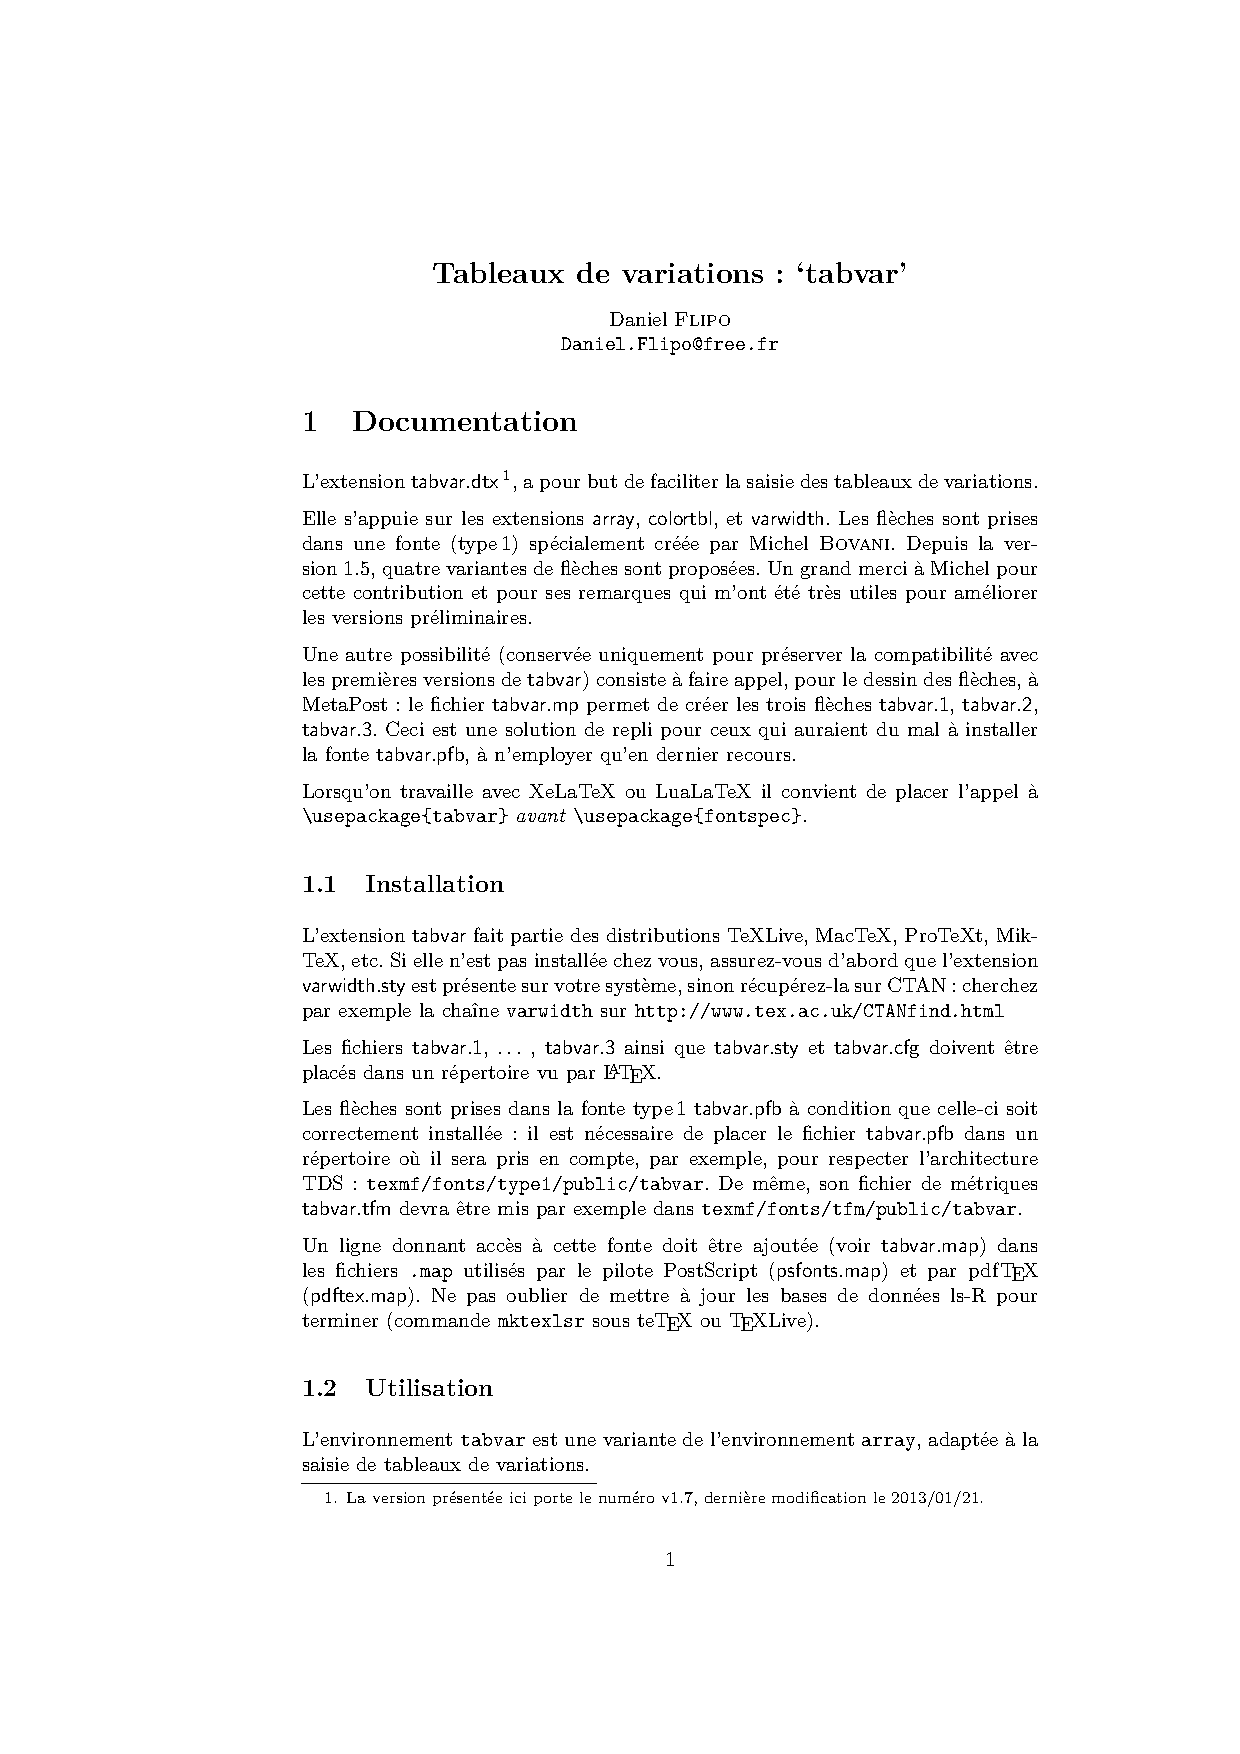
\includegraphics[scale=\TVarrowscale]{tabvar.1}}%
    \sbox{\ardown}{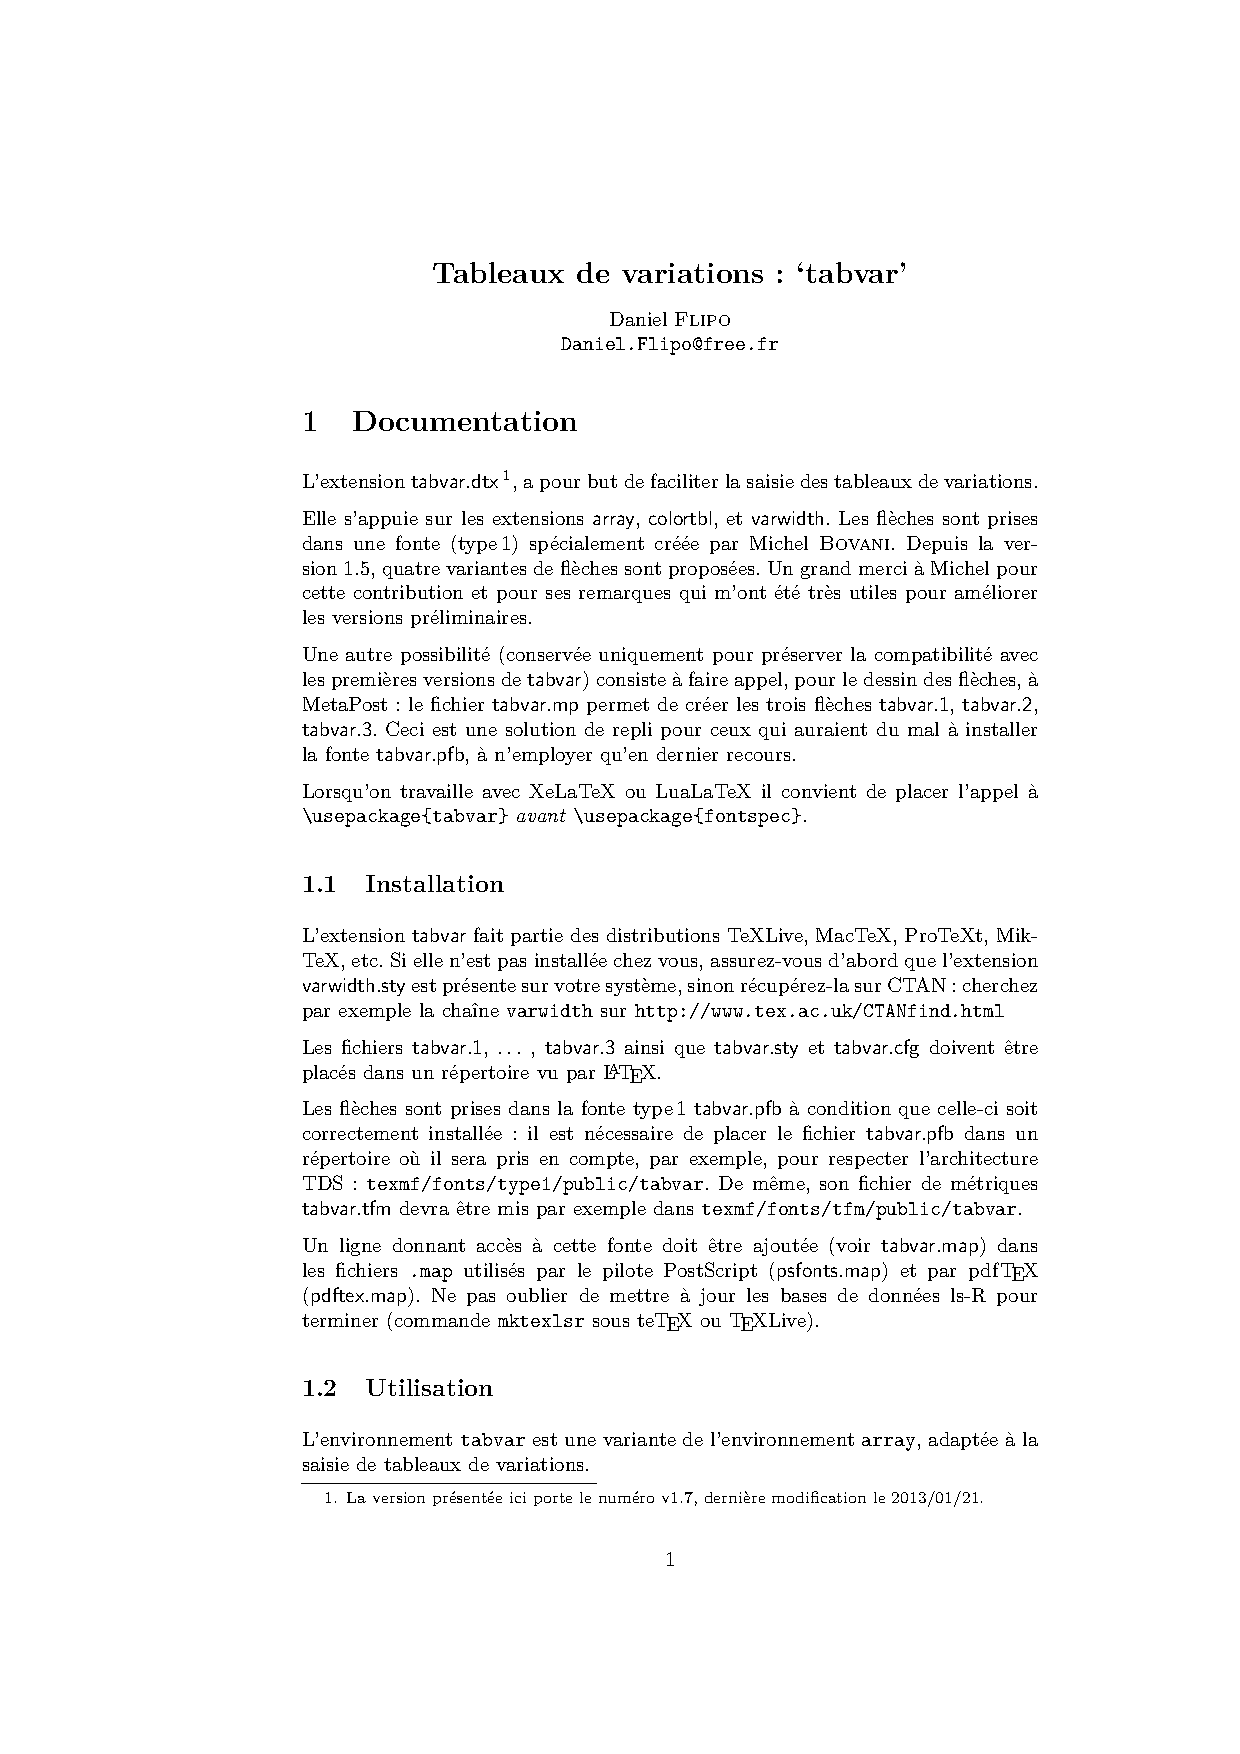
\includegraphics[scale=\TVarrowscale]{tabvar.2}}%
    \sbox{\arhor}{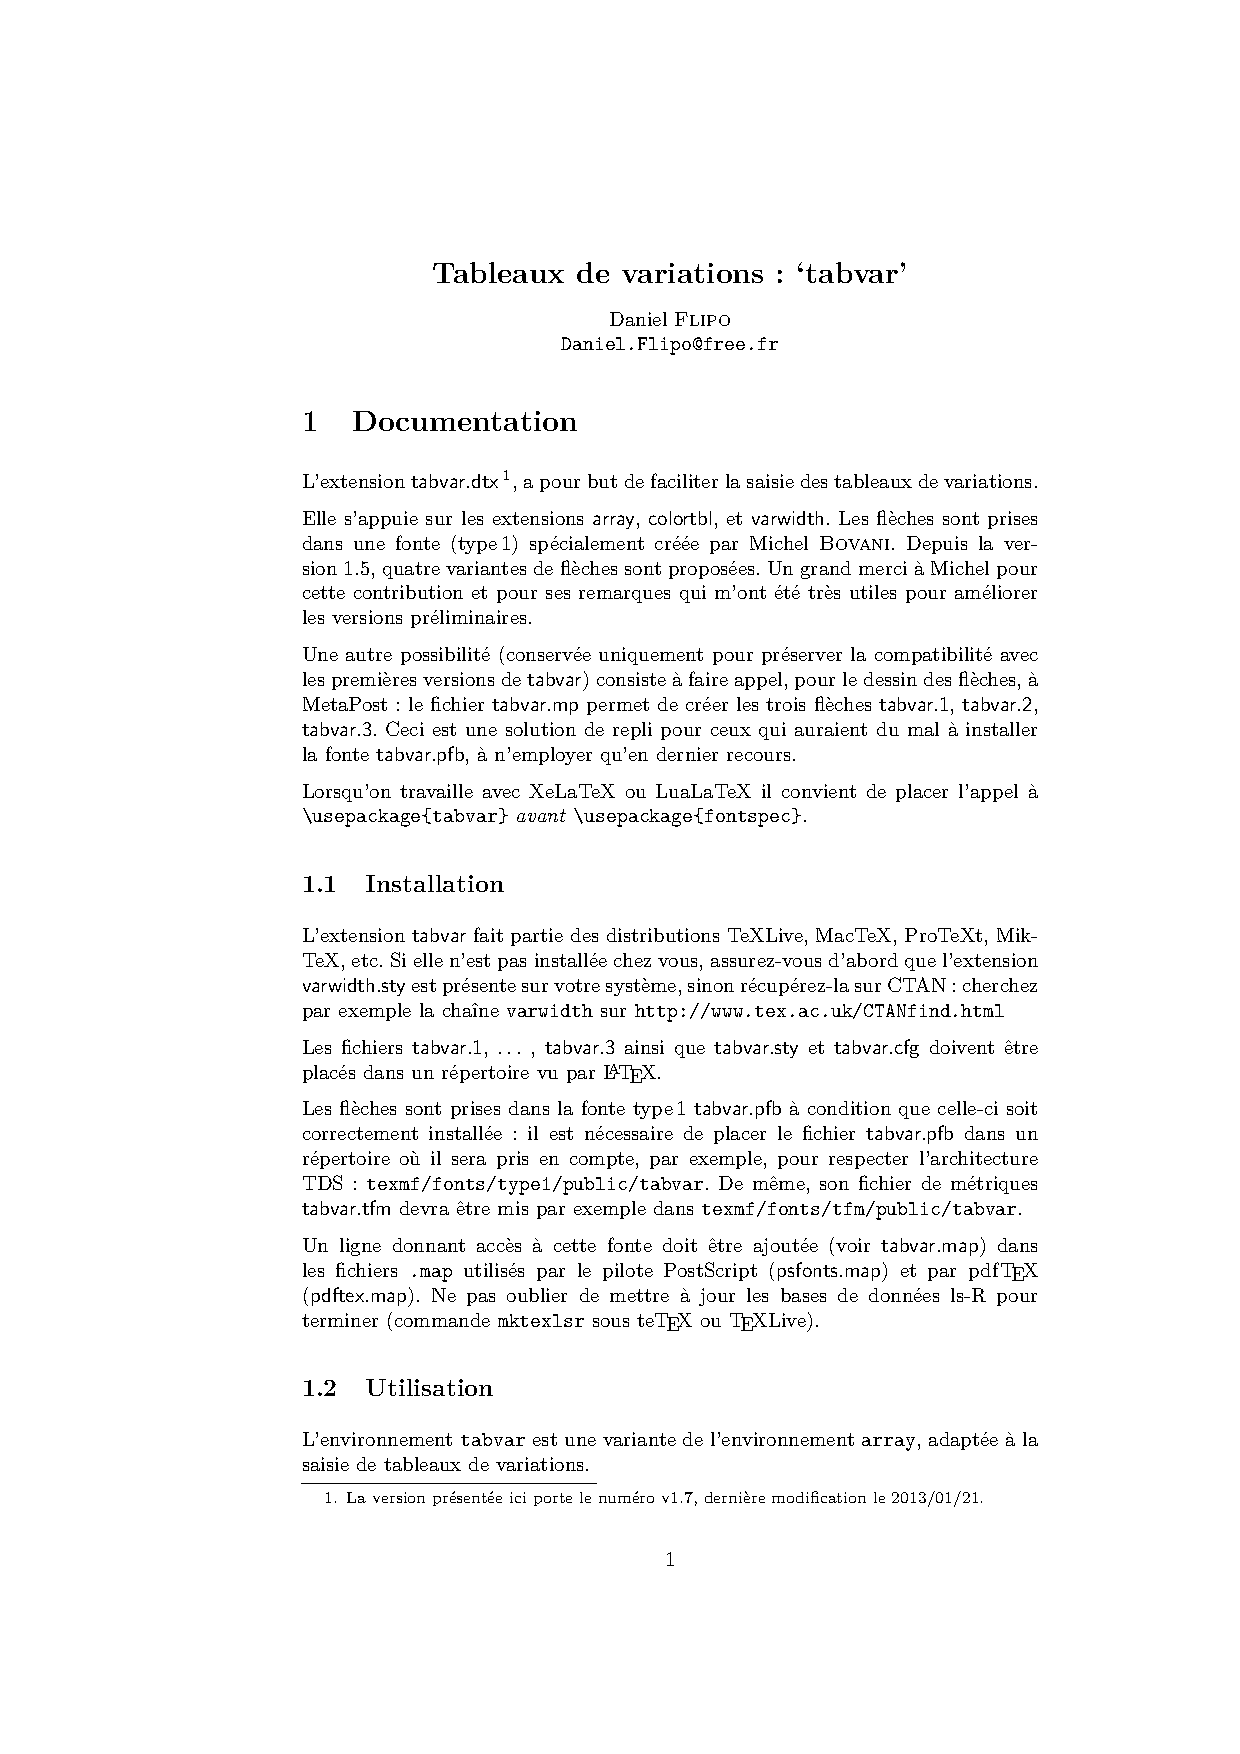
\includegraphics[scale=\TVarrowscale]{tabvar.3}}%
    \newcommand*{\FlecheC}{%
        \TV@arrowcol@stretch{\raisebox{.5ex}{\usebox{\arup}}}}%
    \newcommand*{\FlecheD}{%
        \TV@arrowcol@stretch{\raisebox{.5ex}{\usebox{\ardown}}}}%
    \newcommand*{\FlecheH}{%
        \TV@arrowcol@stretch{\raisebox{.5ex}{\usebox{\arhor}}}}%
  \else
    \DeclareFontFamily{U}{tv}{}%
    \DeclareFontShape{U}{tv}{m}{n}{<->tabvar}{}%
    \DeclareSymbolFont{tvsymbols}{U}{tv}{m}{n}%
    \DeclareMathSymbol{\eastarrowi}{\mathrel}{tvsymbols}{"21}%
    \DeclareMathSymbol{\enearrowi}{\mathrel}{tvsymbols}{"25}%
    \DeclareMathSymbol{\esearrowi}{\mathrel}{tvsymbols}{"26}%
    \DeclareMathSymbol{\eastarrowii}{\mathrel}{tvsymbols}{"31}%
    \DeclareMathSymbol{\enearrowii}{\mathrel}{tvsymbols}{"35}%
    \DeclareMathSymbol{\esearrowii}{\mathrel}{tvsymbols}{"36}%
    \DeclareMathSymbol{\eastarrowiii}{\mathrel}{tvsymbols}{"3B}%
    \DeclareMathSymbol{\enearrowiii}{\mathrel}{tvsymbols}{"3F}%
    \DeclareMathSymbol{\esearrowiii}{\mathrel}{tvsymbols}{"40}%
    \DeclareMathSymbol{\eastarrowiv}{\mathrel}{tvsymbols}{"46}%
    \DeclareMathSymbol{\enearrowiv}{\mathrel}{tvsymbols}{"4A}%
    \DeclareMathSymbol{\esearrowiv}{\mathrel}{tvsymbols}{"4B}%
    \newcommand*{\FlecheC}{%
            \TV@arrowcol@stretch{\ensuremath{\enearrow}}}%
    \newcommand*{\FlecheD}{%
            \TV@arrowcol@stretch{\ensuremath{\esearrow}}}%
    \newcommand*{\FlecheH}{%
            \TV@arrowcol@stretch{\ensuremath{\eastarrow}}}%
  \fi}
%    \end{macrocode}
%  \end{macro}
%  \end{macro}
%  \end{macro}
%
%  \subsection{Positionnement vertical de \'el\'ements}
%
%    La variable |\TVextraheight|, dont la valeur par d\'efaut vaut
%    |.7\baselineskip| permet d'\'ecarter l\'eg\`erement les valeurs
%    maximales de la fonction, du filet horizontal sup\'erieur.
%
%    \begin{macrocode}
\newdimen\TVextraheight
\setlength{\TVextraheight}{.7\baselineskip}
%    \end{macrocode}
%
%  \begin{macro}{\niveau}
%    La commande |\niveau|, utilis\'ee uniquement dans les lignes
%    relatives aux valeurs des fonctions, permet d'initialiser les
%    valeurs des compteurs |\@niveaux| (nombre total de niveaux
%    utilis\'es dans la ligne) et |\@pos| (indicateur du niveau
%    courant). Elle active \'egalement le drapeau |\if@socle|
%    utilis\'e par la commande |\@socle|. Celle-ci place un filet
%    invisible de hauteur |\TVextraheight| et ajoute |\@pos - 1|
%    sauts de lignes (les colonnes sont align\'ees par le bas), ce
%    qui assure le positionnement vertical de l'\'el\'ement (valeur
%    de la fonction ou fl\`eche).
%    Le drapeau |\if@socle| devra \^etre mis localement \`a `faux'
%    dans certaines colonnes (cf. |\dbarre| et |discont|).
%    \begin{macrocode}
\newcount\@niveaux
\newcount\@pos
\newif\if@socle
\newcommand{\niveau}[2]{\global\@pos=#1 \global\@niveaux=#2
                        \global\@socletrue}
\newcommand{\@socle}{%
  \ifnum\@pos=1 \@soclefalse \fi
  \if@socle
    \rule{\z@}{\TVextraheight}%
    \@tempcnta=\@pos
    \advance\@tempcnta by -1
    \whiledo{\@tempcnta>0}{\TVnl \null \advance\@tempcnta by -1}%
  \fi}
%    \end{macrocode}
%  \end{macro}
%
%  \subsection{Nouveaux types de colonnes}
%
%    Ces d\'efinitions n\'ecessitent les extensions |array| et
%    |varwidth|. L'environnement |varwidth|, comme |minipage|,
%    red\'efinit la commande |\\|.  On la renomme \`a l'int\'erieur
%    des environnements |varwidth|, de fa\c{c}on \`a \'eviter la
%    confusion entre passage \`a la ligne \`a l'int\'erieur d'une
%    colonne et passage \`a la ligne suivante du tableau :
%    |\TVnl| (commande interne) provoque un changement de ligne \`a
%    l'int\'erieur d'une colonne, l'utilisateur peut continuer \`a
%    utiliser |\\| pour terminer une ligne du tableau.
%    La commande |\TVtabularnewline|, d\'efinie dans l'environnement
%    \env{tabvar}, provoque un changement de ligne dans le tableau
%    (|\tabularnewline|) et affecte la valeur `vrai' au drapeau
%    |\ifreset@niveaux|, ce qui commande la r\'einitialisation des
%    compteurs |\@pos| et |\@niveaux| \`a la valeur~1.
%    Cette r\'einitialisation aura lieu \emph{apr\`es} que la
%    commande |\@socle| ait plac\'e les valeurs de la fonction et
%    les fl\`eches \`a la bonne hauteur.
%
%    \begin{macrocode}
\newif\ifreset@niveaux
\newcommand{\reset@niveaux}{%
  \ifreset@niveaux
    \global\@niveaux=1 \global\@pos=1 \global\@soclefalse
  \fi}
%    \end{macrocode}
%
% \changes{tabvar-1.0}{2006/03/14}{Ajout d'un param\`etre
%    \cs{TVmaxcolwidth} pour choisir la largeur maximale des colonnes
%    de type C, L, R, au lieu d'une valeur fixe.}
%
% \changes{tabvar-1.2b}{2009/10/03}{Augmenter la valeur de
%    \cs{TVmaxcolwidth} \`a \cs{linewidth}).}
%
%    On d\'efinit des variantes \ctype{C}, \ctype{L} et \ctype{R},
%    des colonnes \ctype{c}, \ctype{l} et \ctype{r} : ce sont des
%    \emph{minipage} align\'ees par le bas, dont la largeur est celle
%    de la ligne la plus longue, avec un maximum de |\TVmaxcolwidth|
%    fix\'e \`a |\linewidth| par d\'efaut, (voir la documentation de
%    l'extension \file{varwidth.sty}).
%
%    \begin{macrocode}
\newdimen\TVmaxcolwidth
\setlength{\TVmaxcolwidth}{\linewidth}
\newcolumntype{C}{%
   >{\begin{varwidth}[b]{\TVmaxcolwidth}\let\TVnl=\\
     \let\\=\TVtabularnewline $}%
   c%
   <{\@socle \reset@niveaux
     $\@finalstrut\@arstrutbox\end{varwidth}}}
\newcolumntype{L}{%
   >{\begin{varwidth}[b]{\TVmaxcolwidth}\let\TVnl=\\
     \let\\=\TVtabularnewline $}%
   l%
   <{\@socle \reset@niveaux
     $\@finalstrut\@arstrutbox\end{varwidth}}}
\newcolumntype{R}{%
   >{\begin{varwidth}[b]{\TVmaxcolwidth}\let\TVnl=\\
     \let\\=\TVtabularnewline $}%
   r%
   <{\@socle \reset@niveaux
     $\@finalstrut\@arstrutbox\end{varwidth}}}
%    \end{macrocode}
%
%\changes{tabvar-1.6}{2011/07/07}{Ajout du type `U' synonyme de `N'
%    utilis\'e par numprint.sty. N.B.: c'est la derni\`ere
%    d\'efinition qui est prise en compte par \cs{newcolumntype},
%    donc celle de numprint si tabvar est charg\'e apr\`es tabvar
%    et inversement (cf. array.dtx).}
%
%    On d\'efinit \'egalement un type \ctype{U} pour les domaines o\`u
%    la fonction n'est pas d\'efinie : la colonne est colori\'ee en
%    faisant appel \`a l'extension \file{colortbl}. La couleur
%    peut \^etre choisie par l'utilisateur, par exemple :\\
%    |\definecolor{TVcolor}{rgb}{0.66, 0.8, 0}| \\
%    donne un vert, voir \file{color.sty} pour la fa\c{c}on de
%    d\'efinir des couleurs. L'ancien nom \ctype{N}, conserv\'e pour
%    la compatibilit\'e ascendante, tant qu'il n'y a pas conflit, mais
%    ne devrait plus \^etre utilis\'e.
%
%    \begin{macrocode}
\definecolor{TVcolor}{gray}{0.7}
\newdimen\TVarraycolsep
\newdimen\TVcolorLeftSep
\newdimen\TVcolorRightSep
\setlength{\TVcolorLeftSep}{\TVarraycolsep}
\setlength{\TVcolorRightSep}{\TVarraycolsep}
\newcolumntype{U}{%
   >{\columncolor{TVcolor}[\TVcolorLeftSep][\TVcolorRightSep]}
   c}
\AtBeginDocument{%
  \@ifundefined{NC@find@N}%
     {\newcolumntype{N}{U}}%
     {\PackageWarning{tabvar}{Le type de colonne N est d\'efini par
                              ailleurs. \MessageBreak Remplacer N par
                              U dans \protect\begin{tabvar}{...N...}
                              \MessageBreak}}%
}
%    \end{macrocode}
%
%  \subsection{Commandes de saisie}
%
%    Les valeurs \`a afficher dans chaque ligne peuvent \^etre
%    saisies directement (|1.4|, |+|, |-|, etc.) comme dans un
%    tableau normal. Les lignes correspondant aux valeurs des
%    fonctions comportent plusieurs \'etages, nous disposons
%    deux compteurs, |\@niveaux| qui contient le nombre total
%    de niveaux (ou \'etages) utilis\'es dans la ligne, |\@pos|
%    qui indique le niveau courant.
%
%  \begin{macro}{\croit}
%  \begin{macro}{\decroit}
%  \begin{macro}{\constante}
%    Les commandes |\croit|,|\decroit|  et |\constante| tracent les
%    fl\`eches \`a la hauteur ad\'equate et mettent \`a jour le
%    compteur |\@pos|. Un message d'erreur est affich\'e lorsque
%    l'une de ces commandes fait sortir de la plage de niveaux
%    d\'eclar\'es par la commande |\niveau|.
%
%    \begin{macrocode}
\newcommand{\decroit}{\FlecheD
                      \global\advance\@pos by -1
                      \ifnum\@pos<1
                      \PackageError{tabvar.sty}%
                        {Les arguments la commande
                         \protect\niveau\space sont incorrects}%
                      \fi}
\newcommand{\croit}  {\raisebox{-\baselineskip}{\FlecheC}%
                      \global\advance\@pos by 1
                      \ifnum\@pos>\@niveaux
                      \PackageError{tabvar.sty}%
                        {Les arguments la commande
                         \protect\niveau\space sont incorrects}%
                      \fi}
\newcommand{\constante}{\FlecheH}
%    \end{macrocode}
%  \end{macro}
%  \end{macro}
%  \end{macro}
%
% \changes{tabvar-1.1}{2007/05/07}{Ajout de la commande \cs{barre}.
%   Ajout de \cs{barre@dth} pour le calcul de la hauteur d'une
%   rang\'ee (utilis\'ee par \cs{barre} et \cs{dbarre}).}
%
%  \begin{macro}{\dbarre}
%    La commande |\dbarre| sert \`a tracer les doubles barres
%    La commande |\vline| ne peut pas \^etre utilis\'ee \`a cette fin
%    dans les environnements de type |\parbox|, car sa port\'ee
%    est limit\'ee \`a un interligne.
%
%    On calcule la hauteur exacte de la rang\'ee, dans les deux cas
%    |\@niveaux=1| et |\@niveaux>1|, |\@tempdimc| contient la hauteur
%    totale (\textit{totalheight}) et |\@tempdimb| la profondeur
%    (\textit{depth}).
%    \begin{macrocode}
\newcommand{\barre@dth}{%
   \ifnum\@niveaux=1
     \@tempdimc=\TVarraystretch\baselineskip
   \else
     \@tempcnta=\@niveaux
     \advance\@tempcnta by -1
     \@tempdimc=\@tempcnta\baselineskip
     \@tempdimb=\TVextraheight
     \ifdim\@tempdimb<.7\baselineskip
       \@tempdimb=.7\baselineskip
     \fi
     \advance\@tempdimc by \@tempdimb
     \advance\@tempdimc by \dp\@arstrutbox
   \fi
   \@tempdimb=\dp\@arstrutbox}
%    \end{macrocode}
%    On fait appel \`a |\rule| pour le trac\'e de |\dbarre|.
%    \begin{macrocode}
\newcommand{\dbarre}{%
   \barre@dth
   \rule[-\@tempdimb]{.5\p@}{\@tempdimc}%
   \kern 2\p@
   \rule[-\@tempdimb]{.5\p@}{\@tempdimc}%
   \@soclefalse}
%    \end{macrocode}
%  \end{macro}
%
%\changes{tabvar-1.3}{2010/04/03}{%
%  Valeur de la profondeur \cs{@tempdimb} corrig\'ee dans \cs{barre}.
%  Bug signal\'e par Frank Stengel.}
%
%  \begin{macro}{\barre}
%    La commande |\barre| prend un argument obligatoire.
%    |\barre{}| trace un filet vertical centr\'e dans une colonne.
%    Lorsque l'argument est non vide, celui-ci est superpos\'e
%    (centr\'e) sur le filet. Le filet est trac\'e en gris
%    par d\'efaut (couleur param\'etrable).
%    \begin{macrocode}
\newsavebox{\tab@box}
\definecolor{TVbarrecolor}{gray}{0.7}
\newcommand{\barre}[1]{%
   \sbox{\tab@box}{\ensuremath{#1}}%
   \barre@dth
   \@tempcnta=\@pos
   \advance\@tempcnta by -1
   \advance\@tempdimb by \@tempcnta\baselineskip
   \raisebox{-\@tempdimb}[0pt][0pt]{%
      \makebox[\wd\tab@box][c]{\color{TVbarrecolor}%
                               \rule{.5\p@}{\@tempdimc}}}%
   \kern-\wd\tab@box\usebox{\tab@box}%
}
%    \end{macrocode}
%  \end{macro}
%
%  \begin{macro}{\discont}
%    La commande |\discont| s'utilise lorsque la fonction pr\'esente
%    une discontinuit\'e, elle r\'eclame 3 arguments obligatoires :
%    le premier est la limite \`a gauche~$f_-$, le deuxi\`eme le signe
%    '<' ou '>', le troisi\`eme est la limite \`a droite~$f_+$.
%    \LaTeX{} ne peut pas toujours comparer facilement les valeurs
%    de $f_-$ et $f_+$ (penser \`a $f_-=\sqrt{e}$, $f_+=\pi/2$), le
%    deuxi\`eme argument pr\'ecise si $f_- < f_+$ ou si $f_- > f_+$.
%
%    En plus de ces 3 arguments obligatoires, un argument optionnel
%    (entier positif) permet d'\'ecarter verticalement les valeurs
%    $f_-$ et~$f_+$ ; la valeur de cet entier donne le nombre de
%    niveaux suppl\'ementaires \`a intercaler (0 par d\'efaut).
%
%    On commence par mesurer la largeur des deux arguments |#2| et
%    |#4| pour pouvoir les centrer ensuite dans une bo\^{\i}te de
%    largeur \'egale au maximum des deux largeurs.
%    Si cette disposition ne convient pas, on pourra toujours
%    ajouter un |\hfill| \`a droite o\`u \`a gauche de la valeur
%    \`a d\'eplacer.
%
%    \begin{macrocode}
\newcommand{\discont}[4][0]{%
     \settowidth{\@tempdimc}{\ensuremath{#2}}%
     \settowidth{\@tempdimb}{\ensuremath{#4}}%
     \ifdim\@tempdimc<\@tempdimb \@tempdimc=\@tempdimb\fi
     \rule{\z@}{\TVextraheight}%
     \@soclefalse
     \ifthenelse{\equal{#3}{<}}%
%    \end{macrocode}
%    Cas o\`u $f_- < f_+$ : on pose la valeur de~$f_+$ (|#4|), puis
%    on saute autant de lignes suppl\'ementaires qu'indiqu\'e dans
%    l'argument optionnel, ensuite on passe \`a la ligne et on pose
%    la valeur de~$f_-$ (|#2|), enfin on ajoute en dessous
%    |\@pos - 1| sauts de lignes pour positionner le tout en hauteur.
%    Il reste \`a ajuster le compteur~|\@pos| pour que la fl\`eche
%    suivante soit plac\'ee \`a la bonne hauteur.
%    \begin{macrocode}
     {\makebox[\@tempdimc]{\ensuremath{#4}}%
      \@tempcnta=#1
      \whiledo{\@tempcnta>0}{\TVnl \null \advance\@tempcnta by -1}%
      \TVnl
      \makebox[\@tempdimc]{\ensuremath{#2}}%
      \@tempcnta=\@pos
      \advance\@tempcnta by -1
      \whiledo{\@tempcnta>0}{\TVnl \null \advance\@tempcnta by -1}%
      \global\advance\@pos by 1
      \global\advance\@pos by #1
     }%
     {\ifthenelse{\equal{#3}{>}}%
%    \end{macrocode}
%    Cas o\`u $f_- > f_+$ : \textit{idem} en permutant $f_-$ et~$f_+$.
%    \begin{macrocode}
     {\makebox[\@tempdimc]{\ensuremath{#2}}%
      \@tempcnta=#1
      \whiledo{\@tempcnta>0}{\TVnl \null \advance\@tempcnta by -1}%
      \TVnl
      \makebox[\@tempdimc]{\ensuremath{#4}}%
      \@tempcnta=\@pos
      \advance\@tempcnta by -2
      \advance\@tempcnta by -#1
      \whiledo{\@tempcnta>0}{\TVnl \null \advance\@tempcnta by -1}%
      \global\advance\@pos by -1
      \global\advance\@pos by -#1
     }%
%    \end{macrocode}
%    Cas o\`u le deuxi\`eme argument n'est ni |<| ni |>| : erreur
%    \begin{macrocode}
     {\PackageError{tabvar.sty}%
        {Le second argument de \protect\discont\space doit \^etre
         \MessageBreak soit '<' soit '>'}}%
     }%
}
%    \end{macrocode}
%  \end{macro}
%
%\changes{tabvar-1.6}{2011/07/07}{Ajout de la commande \cs{TVcenter}.}
%
%  \begin{macro}{\TVcenter}
%    La commande |\TVcenter{}| prend un argument, le nom de la
%    fonction \`a centrer verticalement dans sa colonne.
%    \begin{macrocode}
\newcommand*{\TVcenter}[1]{%
  \@tempcnta=\@niveaux \advance\@tempcnta by -1 \divide\@tempcnta by 2
  \@tempdimb=\@tempcnta\baselineskip
  \ifodd\@niveaux\else\advance\@tempdimb by .5\baselineskip\fi
  \@pos=1\raisebox{\@tempdimb}{\ensuremath{#1}}%
}
%    \end{macrocode}
%  \end{macro}
%
%\changes{tabvar-1.7}{2012/12/23}{Ajout de la commande \cs{TVstretch}.}
%
%  \begin{macro}{\TVstretch}
%    La commande |\TVstretch{}| prend un argument obligatoire, le nom
%    de la valeur \`a \'ecarter des lignes horizontales et un
%    argument optionnel de type \emph{dimension}.
%    Elle place son argument dans une bo\^{\i}te et en mesure la hauteur
%    et la profondeur. En l'absence d'argument optionnel, elle ajoute
%    respectivement |\TVextraheight| \`a la hauteur |\TV@tempa| et
%    |\TVextradepth| \`a la profondeur |\TV@tempb|.
% 
%    Si l'argument optionnel est une dimension positive, sa valeur
%    sera ajout\'ee uniquement \`a la hauteur et si c'est une
%    dimension n\'egative sa valeur absolue sera ajout\'ee uniquement
%    \`a la profondeur. La valeur par d\'efaut de l'argument optionnel
%    est |0pt|.
%
%    \begin{macrocode}
\newsavebox\TVbox
\newdimen\TVextraheight
\newdimen\TVextradepth
\setlength{\TVextraheight}{2pt}
\setlength{\TVextradepth}{2pt}
\newdimen\TV@tempa
\newdimen\TV@tempb
\newcommand{\TVstretch}[2][0pt]{%
  \edef\tmp{#1}%
  \sbox{\TVbox}{\ensuremath{#2}}%
  \settoheight{\TV@tempa}{\usebox{\TVbox}}%
  \settodepth {\TV@tempb}{\usebox{\TVbox}}%
  \ifdim\tmp=0pt
    \addtolength{\TV@tempa}{\TVextraheight}%
    \addtolength{\TV@tempb}{\TVextradepth}%
  \else
    \ifdim\tmp>0pt
      \addtolength{\TV@tempa}{\tmp}%
    \else
      \addtolength{\TV@tempb}{-\tmp}%
    \fi
  \fi
%    \end{macrocode}
%    Il reste \`a afficher la bo\^{\i}te initiale et \`a lui adjoindre
%    une |\rule| invisible (de largeur nulle) de profondeur
%    |\TV@tempb| et de hauteur totale |\TV@tempa + \TV@tempb|.
%    \begin{macrocode}
  \usebox{\TVbox}%
  \addtolength{\TV@tempa}{\TV@tempb}%
  \rule[-\TV@tempb]{0pt}{\TV@tempa}%
}
%    \end{macrocode}
%  \end{macro}
%
%  \subsection{Environnement `tabvar'}
%
%    L'environnement \env{tabvar} est un \env{array} o\`u sont
%    red\'efinis |\TVarraystretch|, |\TVarraycolsep| et
%    |\tabularnewline|.
%
%  \begin{environment}{tabvar}
%    \begin{macrocode}
\newcommand{\TVarraystretch}{1.5}
\setlength{\TVarraycolsep}{1pt}
\newenvironment{tabvar}[1]
  {\renewcommand{\arraystretch}{\TVarraystretch}%
   \setlength{\arraycolsep}{\TVarraycolsep}%
   \global\@niveaux=1 \global\@pos=1 \global\@soclefalse
   \def\TVtabularnewline{\reset@niveauxtrue\tabularnewline}%
   \begin{array}{#1}}
  {\end{array}}
%    \end{macrocode}
%  \end{environment}
%
%    Chargement du fichier de pr\'ef\'erences, si il en existe un.
%    \begin{macrocode}
\InputIfFileExists{tabvar.cfg}
   {\typeout{loading tabvar.cfg}}
   {\typeout{tabvar.cfg not found, using default values}}
%    \end{macrocode}
% \iffalse
%</sty>
% \fi
%
%  \section{Fichier de configuration}
%
% \iffalse
%<*cfg>
% \fi
%    \begin{macrocode}
%% Fichier de configuration de l'extension `tabvar.sty'.
%%
%% D\'ecommenter la ligne suivante pour que les variantes MetaPost
%% des fl\`eches soient utilis\'ees \`a la place de la fonte tabvar.pfb
%% (d\'econseill\'e en g\'en\'eral et *jamais* sous LuaLaTeX ou XeLaTeX).
%%
%%\FlechesMPtrue
%%
%% Choix d'une des 4 variantes pour les fl\`eches PostScript
%%
%%\FlechesPS1   % (d\'efaut)
%%\FlechesPS2   % assorties \`a la police Fourier
%%\FlechesPS3
%%\FlechesPS4
%%
%% Ce param\`etre permet d'augmenter la largeur des colonnes contenant
%% des fl\`eches (essayer 1.3, 1.5, etc.), sa valeur par d\'efaut est 1 :
%%
%%\renewcommand*{\TVarrowscolstretch}{1}
%%
%% Ce param\`etre permet d'ajuster la hauteur des lignes
%% de `tabvar' correspondant aux variations d'une fonction ;
%% sa valeur par d\'efaut est :
%%
%%\setlength{\TVextraheight}{0.7\baselineskip}
%%
%% Valeur de \arraycolsep utilis\'ee dans `tabvar'.
%%
%%\setlength{\TVarraycolsep}{1pt}
%%
%% Valeur de \arraystretch utilis\'ee dans `tabvar'.
%%
%%\renewcommand{\TVarraystretch}{1.5}
%%
%% Largeur maximale des colonnes de type C, L ou R.
%%
%%\setlength{\TVmaxcolwidth}{\linewidth}
%%
%% Valeur des espaces verticaux ajout\'es par la commande
%% |\TVstretch{}|.
%%
%%\setlength{\TVextraheight}{2pt}
%%\setlength{\TVextradepth}{2pt}
%%
%% Exemples de d\'efinitions de couleurs pour les colonnes `U'
%% o\`u la fonction est non d\'efinie.
%%
%%\definecolor{TVcolor}{gray}{0.5}
%%\definecolor{TVcolor}{rgb}{0.33, 0.12, 0}
%%\definecolor{TVcolor}{cmyk}{0.91,0,0.88,0.12}
%%
%% Les valeurs suivantes assurent que les colonnes `U' sont
%% colori\'ees sur toute leur largeur.
%%
%%\setlength{\TVcolorLeftSep}{\TVarraycolsep}
%%\setlength{\TVcolorRightSep}{\TVarraycolsep}
%%
%% On peut ajuster comme ci-dessus la couleur des filets
%% tra\c{c}\'es par la commande \barre{}.
%%
%%\definecolor{TVbarrecolor}{gray}{0.7}
%    \end{macrocode}
% \iffalse
%</cfg>
% \fi
%
% \Finale
%
% \PrintChanges
\endinput

%%% Local Variables:
%%% fill-column: 70
%%% coding: us-ascii
%%% End:
